\clearpage

\vspace*{-1\baselineskip}
\section{等待CSMA的设计及分析}
\vspace{6pt}

第三章已经在时隙 ALOHA 中引入了等待随机接入退避机制，并给出了相应的理论分析。若进一步将这一思路推广到标准 CSMA 网络中的话，问题就不仅只是“是否发送”，而且还要处理载波侦听、退避计时器冻结与恢复等机制带来的影响。换言之，等待机制仍然用于改善信息时效性，但其协议形式和分析方法都需要结合标准 CSMA 的竞争规则重新建立。

本章内容的安排如下：4.1 节给出等待 CSMA 的系统模型、AoI 演化规律以及退避规则，并说明其与第三章模型的主要区别；4.2 节基于马尔可夫链建立稳态接入模型，推导碰撞概率的稳态方程，并讨论其解的存在性与唯一性；4.3 节在此基础上推导平均 AoI 与 AoI 违规概率的闭式表达；4.4 节结合所得结果讨论等待窗口对系统性能的影响；4.5 节对本章工作进行总结。

\subsection{系统模型}

本章考虑一个由单个 AP 和 $N$ 个终端组成的无线网络。与第三章采用时隙 ALOHA 不同，这里的终端按照标准 CSMA 的方式接入共享信道，即终端在发送前先进行载波侦听，并通过随机退避计时器协调竞争过程。

标准 CSMA 采用基于载波侦听的分布式接入方式。终端在准备发送数据前，会先侦听无线信道；当信道空闲时，终端进入退避阶段，从竞争窗口中随机选取一个整数退避值，并以微时隙为单位开始倒数。若当前微时隙内信道保持空闲，则退避计时器减 1；若有其他终端开始发送，则信道转为忙碌，当前终端立即冻结其退避计时器，待该次忙碌传输结束且信道重新空闲后，退避计时器再恢复计数。计时器减至零的终端获得发送机会，若多个终端在同一时刻归零，则该时刻内发送包的终端将发生碰撞，发送失败。由此可见，标准 CSMA 的核心不只是随机退避本身，还包括“侦听、冻结、恢复与发送”这一循环竞争过程，如图\ref{fig:cp4_csma_and_system_slot}所示。
\begin{figure}[htbp]
\centering
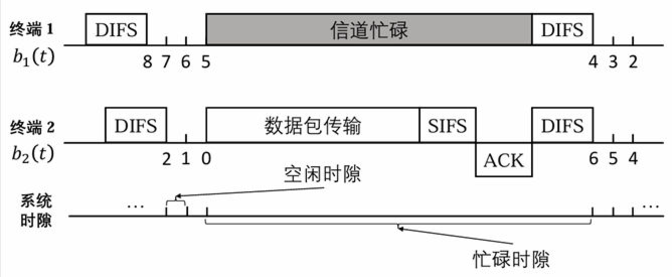
\includegraphics[width=0.8\textwidth]{figure/cp4/CSMA机制与系统时隙的图示.pdf}
\caption{CSMA 机制与系统时隙的图示}
\label{fig:cp4_csma_and_system_slot}
\end{figure}

为了与上述机制的演化过程相匹配，本文不再沿用第三章中的等长时隙设定，而是将每一次退避计时器可能发生变化的时间边界定义为一个系统时隙。这样定义的好处在于，退避计时器的演化可以直接与信道状态对应起来。当所有终端的退避计时器都大于零时，当前系统时隙对应一个空闲微时隙，所有仍处于竞争中的终端同步完成一次倒计时；当终端的计时器归零并开始发送后，系统便会进入忙碌阶段，在这段时间内其余终端的退避计时器全部冻结，直到该忙碌阶段结束后才会进入下一次的更新。因此，系统时隙在物理时间上并不是固定长度，而是取决于当前信道究竟处于空闲还是忙碌的状态。记归一化后的空闲系统时隙长度为 $\frac{1}{M}$，忙碌系统时隙长度为 1，即一次数据传输的持续时间是微时隙的 $M$ 倍，则第 $t$ 个系统时隙的长度 $d(t)$ 可表示为
\begin{equation}
    d(t) =
\begin{cases}
\frac{1}{M}, & \text{if } b_i(t) \neq 0, \forall i, \\
1, & \text{if } b_i(t) = 0, \exists i.
\end{cases}
\end{equation}

与第三章相同，本文仍然采用按需生成的采样机制。终端仅在决定发起传输时才对物理过程进行采样并生成新的状态更新包，因此发送端的排队时延可以忽略不计。根据 AoI 的定义，终端 $i$ 在第 $t$ 个系统时隙的 AoI 演化为
\begin{equation}
    \Delta_i(t + 1) =
\begin{cases}
\Delta_i(t) + \dfrac{1}{M}, & \text{if } b_i(t) \neq 0, \, b_j(t) \neq 0 \, \forall j, \\
1, & \text{if } b_i(t) = 0, \, b_j(t) \neq 0 \, \forall j, \\
\Delta_i(t) + 1, & \text{if } b_j(t) = 0 \, \exists j.
\end{cases}
\end{equation}
三种情形分别对应空闲系统时隙、终端 $i$ 成功传输，以及系统时隙内存在其他终端发送或发生碰撞。该模型下 AoI 的典型演化轨迹如图\ref{fig:cp4_csma_aoi_evolution}所示。
\begin{figure}[htbp]
\centering

\includegraphics[width=0.8\textwidth]{figure/cp4/AoI变化趋势图.pdf}
\caption{AoI 变化趋势图}
\label{fig:cp4_csma_aoi_evolution}
\end{figure}

在大规模接入场景中，CSMA 网络同样面临着与第三章类似的问题：刚完成更新的终端在短时间内继续占用信道，对降低 AoI 的帮助十分有限；而那些长期未成功传输的终端，其在接收端处的状态信息往往已经过时。基于这一点，本文将等待随机接入退避机制引入标准 CSMA，构造等待 CSMA 协议。其规则如下：

1.\textbf{成功传输后的混合退避。} 当终端成功完成一次状态更新后，不再像第三章那样只经历固定的 $z$ 个时隙等待后立即重新接入信道，而是先等待 $z$ 个时隙，再从区间 $[0,w-1]$ 中随机选择一个退避计时器 $\beta$。也就是说，新的退避计时器落在区间 $[z,z+w-1]$ 上。其中，参数 $z$ 用于抑制刚完成更新的终端在短时间内重新参与竞争，而随机退避部分则保留了标准 CSMA 原有的接入机制，用于降低碰撞概率。

2.\textbf{碰撞后的随机退避。} 当终端发送失败时，仍按照标准 CSMA 的方式随机生成 $\beta \sim \text{unif}(0,w-1)$ 的退避计时器，以降低后续重复碰撞的概率。

据此，终端 $i$ 在第 $t$ 个系统时隙的退避计时器满足
\begin{equation}\label{cp4_backoff_counter_evolution}
    b_i(t + 1) =
\begin{cases}
z + \beta, & \text{if } b_i(t) = 0, \, b_j(t) \neq 0 \ \forall j, \\
\beta, & \text{if } b_i(t) = 0, \, b_j(t) = 0 \ \exists j, \\
b_i(t) - 1, & \text{if } b_i(t) \neq 0.
\end{cases}
\end{equation}
式中，$b_j(t)$ 表示除终端 $i$ 之外的其他终端在 $t$ 时刻下的退避计时器状态。

根据第二章的统一分析框架，平均 AoI 与 AoI 违规概率的计算最终仍然归结为相邻两次成功更新之间的离开时间间隔 $Y$。不过，与第三章不同，这里的 $Y$ 不仅受到碰撞与退避的影响，还会受到系统时隙变长的影响。为了避免多终端联合的状态空间所带来的复杂性，本文继续采用 Bianchi 的解耦假设：当终端数量足够大且系统进入稳态后，目标终端在任一系统时隙内感知到的碰撞概率 $p$ 可近似视为常数，各终端行为在统计意义下相互独立。

\subsection{基于马尔可夫链的稳态接入分析}

在等待 CSMA 中，目标终端是否遭遇碰撞取决于其他终端是否在同一系统时隙内进行发送，因此稳态碰撞概率 $p$ 是本章分析的关键参数。本节先构造目标终端的马尔可夫链模型，再建立发送状态与碰撞概率之间的稳态方程，并讨论其解的存在性与唯一性。

\subsubsection{状态转移模型}

第三章分析等待 ALOHA 时，采用了二维马尔可夫链 $(m(t),n(t))$ 对退避计时器和 AoI 的联合演化过程进行建模。对等待 CSMA 而言，若仍然沿用这一思路，则不仅需要描述退避计时器状态，还要处理系统时隙变长所带来的额外复杂性，状态空间会迅速增大。

不过，与第三章不同的是，这里没有必要把退避状态和 AoI 演化放在同一个马尔可夫链中联合刻画。对等待 CSMA 而言，终端何时发起传输主要由退避计时器的演化所决定，而平均 AoI 与违规概率则可以在得到离开时间间隔 $Y$ 的统计特性后再单独求出。基于这一点，本节只需围绕目标终端的退避计时器建立一维的离散时间马尔可夫链，用来描述 MAC 层的竞争过程。

\begin{figure}[htbp]
\centering
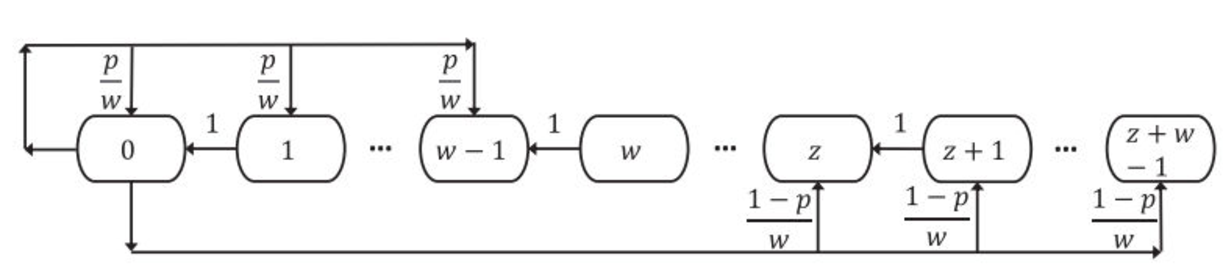
\includegraphics[width=0.92\textwidth]{figure/cp4/马尔可夫链.pdf}
\caption{目标终端的状态转移图}
\label{fig:cp4_mc_chain}
\end{figure}

记
\begin{equation}
    s_l = \lim_{t\to+\infty}\Pr\{b(t)=l\}, \qquad l\in[0,z+w-1]
\end{equation}
为目标终端处于状态 $l$ 的稳态概率。图\ref{fig:cp4_mc_chain}给出了该马尔可夫链的状态转移关系。记 $T_{m,n}$ 为从状态 $s_m$ 到状态 $s_n$ 的转移概率。根据式\eqref{cp4_backoff_counter_evolution}，其转移规则可概括为三类：

1. 当目标终端处于状态 $s_0$ 且发送成功时，它将在区间 $[z,z+w-1]$ 内重新选择退避计时器。由于成功概率为 $1-p$，故对应状态的转移概率为 $\frac{1-p}{w}$。

2. 当目标终端处于状态 $s_0$ 且发生碰撞时，它将在区间 $[0,w-1]$ 内重新选择退避计时器。由于碰撞概率为 $p$，故对应状态的转移概率为 $\frac{p}{w}$。

3. 当目标终端处于非零状态时，退避计时器按系统时隙逐步减 1，因此系统将以概率 1 从 $s_m$ 转移到 $s_{m-1}$。

于是，图\ref{fig:cp4_mc_chain}中的转移关系可写为
\begin{equation}\label{cp4_tmn}
    \begin{cases}
T_{0,n} = \frac{1-p}{w}, & \text{if } z \le n \le z + w - 1, \\
T_{0,n} = \frac{p}{w}, & \text{if } 0 \le n \le w - 1, \\
T_{m,m-1} = 1, & \text{if } m \neq 0.
\end{cases}
\end{equation}

\subsubsection{稳态方程的构建}

根据式\eqref{cp4_tmn}与图\ref{fig:cp4_mc_chain}的结构，目标终端在各状态上的稳态概率可以分两种情况写出。

1. 当 $z\ge w$ 时，有
\begin{equation}\label{cp4_zgew}
        s_l =
\begin{cases}
s_0 \left[ (1 - p) + \frac{p(w-l)}{w} \right], & \text{if } 0 \le l \le w - 1, \\
s_0 (1 - p), & \text{if } w \le l < z, \\
\frac{s_0 (1-p)(w+z-l)}{w}, & \text{if } z \le l \le z + w - 1.
\end{cases}
    \end{equation}

2. 当 $z<w$ 时，有
    \begin{equation}\label{cp4_zlw}
        s_l =
\begin{cases}
s_0 \left[ (1 - p) + \dfrac{p(w-l)}{w} \right], & \text{if } 0 \le l \le z - 1, \\
s_0 \left[ \dfrac{(1-p)(z+w-l)}{w} + \dfrac{p(w-l)}{w} \right], & \text{if } z \le l < w, \\
\dfrac{s_0 (1-p)(z+w-l)}{w}, & \text{if } w \le l \le z + w - 1.
\end{cases}
    \end{equation}

将式\eqref{cp4_zgew}和式\eqref{cp4_zlw}分别代入归一化条件 $\sum_{l=0}^{z+w-1}s_l=1$ 中，可统一得到
\begin{equation}\label{cp4_s_0_and_p}
    s_0+z(1-p)s_0+\frac{s_0(w-1)}{2}=1
\end{equation}

这里的 $s_0$ 正是目标终端在一个系统时隙边界处具备发送资格的概率。在包含 $N$ 个终端的网络中，若假设各终端的稳态行为相互独立，则目标终端发生碰撞的条件是其余 $N-1$ 个终端中至少有一个也同时处于状态 0。因此，碰撞概率满足
\begin{equation}\label{cp4_p_and_s0}
    p=1-(1-s_0)^{N-1}.
\end{equation}

将式\eqref{cp4_p_and_s0}代入式\eqref{cp4_s_0_and_p}，消去中间变量 $s_0$，可得到关于 $p$ 的稳态方程
\begin{equation}\label{cp4_ziqiafangcheng_p}
    \left[ 1 + z(1-p) + \frac{w-1}{2} \right] \left( 1 -\sqrt[N -1]{1-p} \right) - 1=0.
\end{equation}
与第三章相比，这一稳态方程的表达形式有所变化。这是因为在等待 CSMA 中，终端成功更新后并不是直接回到固定的等待状态，而是先等待 $z$ 个时隙后，再进入随机退避竞争。与此同时，系统的时隙长度还会随信道状态而变化，因此，这里不能直接沿用第三章中的写法及论证方式，在下一小节将重新讨论解的存在性与唯一性。

\subsubsection{稳态方程解的存在唯一性论证}

尽管式\eqref{cp4_ziqiafangcheng_p}的形式不同于第三章中的稳态方程，但仍可通过变量代换的方式来说明其在定义域 $(0,1)$ 上解的存在性与唯一性。为此，引入中间变量 $x=\sqrt[N-1]{1-p}$。由于 $0<p<1$，故有 $0<x<1$。此时式\eqref{cp4_ziqiafangcheng_p}可改写为
\begin{equation}\label{cp4_ziqiafangcheng_x}
    \left(zx^{N-1}+\frac{w+1}{2}\right)(1-x)=1.
\end{equation}

将 $z$ 分离，可得
\begin{equation}\label{cp4_ziqiafangcheng_z}
    z=\frac{2-(w+1)(1-x)}{2x^{N-1}(1-x)}.
\end{equation}
记式\eqref{cp4_ziqiafangcheng_z}右端为 $H(x)$。由于 $z>0$，则必须有 $2-(w+1)(1-x)>0$，换言之，$x$ 必须满足 $\frac{w-1}{w+1}<x<1$。

首先讨论解的存在性，当 $x\to \left(\frac{w-1}{w+1}\right)^+$ 时，$H(x)$ 的分子趋于 0 且分母为正，因此 $H(x)\to 0$；当 $x\to 1^-$ 时，分母趋于 0 而分子趋于 1，因此 $H(x)\to +\infty$。由于 $H(x)$ 在区间 $\left(\frac{w-1}{w+1},1\right)$ 内连续，根据介值定理，对于任意 $z>0$，至少存在一个 $x^\star$，使得 $H(x^\star)=z$，因此式\eqref{cp4_ziqiafangcheng_p}至少存在一个解。

接下来再讨论解的唯一性。对 $H(x)$ 求导，有
\begin{equation}
    H'(x) = \frac{x^{N-2}}{\left[x^{N-1}(1-x)\right]^2} \cdot Q(x)
\end{equation}
其中
\begin{equation}
    Q(x) = \frac{(w-1)(N-1)}{w+1}x^2 + \left[N - \frac{2(w-1)(N-1)}{w+1}\right]x - \frac{2(N-1)}{w+1}.
\end{equation}
由于 $H'(x)$ 前面的分式恒为正，因此 $H(x)$ 的单调性完全由二次函数 $Q(x)$ 所决定。为了保证 $H(x)$ 能够单调递增，只需要保证 $Q(x)$ 与实轴没有交点，即其判别式满足
\begin{equation}
    \Delta = N^2 - \frac{4(N-1)(w-1)}{w+1}<0.
\end{equation}
整理后可得
\begin{equation}\label{cp4_w}
    w>\frac{N^2-2N+2}{2(N-1)}>\frac{N-1}{2}.
\end{equation}

因此，当式\eqref{cp4_w}成立时，$H(x)$ 在定义区间内单调递增，式\eqref{cp4_ziqiafangcheng_p}存在唯一解。这里得到的唯一性条件与第三章不同，第三章中的条件直接涉及等待窗口 $z$，而本章的条件只由 $N$ 和 $w$ 决定。在满足式\eqref{cp4_w}的条件下，可采用二分法对变量 $x$ 进行求解，再由 $p=1-x^{N-1}$ 得到唯一的稳态碰撞概率。

\subsection{信息时效性指标的理论解析}

在确定稳态碰撞概率 $p$ 后，便可进一步分析等待 CSMA 下的平均 AoI 与 AoI 违规概率。与第三章一样，这里的求解路径仍然是先求离开时间间隔 $Y$ 的一阶矩和二阶矩，再代入第二章的统一公式。不同之处在于，等待 CSMA 中成功更新后的终端并不是简单返回到固定等待状态，而是先等待 $z$ 个时隙，再进入标准 CSMA 的随机退避竞争。同时，系统的时隙长度也会随信道状态而变化，因此 $Y$ 的构成方式与第三章并不相同。

\subsubsection{平均AoI的闭式推导}

在按需生成的采样机制下，每次成功更新后 AoI 都被重置为 1，因此平均 AoI 的计算公式仍可重写为
\begin{equation}\label{cp4_avg_aoi}
    \Delta = 1 + \frac{E[Y^2]}{2E[Y]}.
\end{equation}
其中，$Y$ 表示相邻两次成功更新之间的离开时间间隔。因此，平均 AoI 的推导仍可归结为求解 $Y$ 的一阶矩和二阶矩。与第三章不同，系统时隙的长度会随信道状态而变化，因此求解上更为复杂。

1. 求解 $Y$ 的一阶矩

    设在一个离开时间间隔 $Y$ 内，目标终端共发起 $\alpha$ 次传输尝试。由于每次尝试的碰撞概率均为常数 $p$，故 $\alpha$ 服从参数为 $1-p$ 的几何分布，其概率质量函数为
    \begin{equation}\label{cp4_alpha}
        \Pr\{\alpha=k\}=(1-p)p^{k-1}, \quad k=1,2,\dots
    \end{equation}

    与第三章相比，这里的离开时间间隔由等待阶段和竞争阶段共同构成。为便于求矩，本文将 $Y$ 分解为两部分：$U$ 表示终端成功更新后等待 $z$ 个系统时隙所对应的时间，$V$ 表示终端完成一次发送尝试所经历的竞争时间。

    在本文采用的系统时隙设定下，等待阶段中的单个系统时隙以概率 $p$ 对应长度为 1 的忙碌时隙，以概率 $1-p$ 对应长度为 $\frac{1}{M}$ 的空闲微时隙，因此有
    \begin{equation}\label{cp4_EU}
        E[U] = z\left(p+\frac{1-p}{M}\right).
    \end{equation}

    对于竞争阶段，终端先从区间 $[0,w-1]$ 内随机选取退避计时器 $\beta$，再经历对应的倒计时过程并完成一次发送尝试。于是
    \begin{equation}\label{cp4_EV}
        E[V] = 1 + \sum_{\beta=0}^{w-1}\frac{\beta}{w}\left(p+\frac{1-p}{M}\right)
        = 1+\frac{w-1}{2}\left(p+\frac{1-p}{M}\right).
    \end{equation}

    若在相邻的两次成功更新之间，前 $k-1$ 次尝试均碰撞，第 $k$ 次尝试成功，将对应的离开时间间隔记为 $Y_k$，则根据等待 CSMA 的工作机制，有 $Y_k = U+\sum_{j=1}^{k}V_j$，因此
    \begin{equation}\label{cp4_EYk}
        E[Y_k] = z \left( p + \frac{1-p}{M} \right) + k \left[ 1 + \frac{w-1}{2} \left( p + \frac{1-p}{M} \right) \right].
    \end{equation}

    将式\eqref{cp4_alpha}与式\eqref{cp4_EYk}联立，可得
    \begin{equation}\label{cp4_EY}
        \begin{aligned}
        E[Y] &= \sum_{k=1}^{\infty} \Pr\{\alpha = k\} E[Y_k] \\
        &= z \left( p + \frac{1-p}{M} \right) \sum_{k=1}^{\infty} (1-p) p^{k-1} \\
        &\quad + \left[ 1 + \frac{w-1}{2} \left( p + \frac{1-p}{M} \right) \right] \sum_{k=1}^{\infty} k (1-p) p^{k-1} \\
        &= z \left( p + \frac{1-p}{M} \right) + \frac{1}{1-p} + \frac{\left( p + \frac{1-p}{M} \right) (w-1)}{2(1-p)}.
        \end{aligned}
    \end{equation}

2. 求解 $Y$ 的二阶矩

    为了简化后续书写，记 $\phi=z\left(p+\frac{1-p}{M}\right)$，$\gamma=\frac{w-1}{2}\left(p+\frac{1-p}{M}\right)$。

    在成功后的强制等待阶段，$z$ 个系统时隙中可能出现忙碌时隙和空闲时隙。设其中有 $i$ 个系统时隙为忙碌时隙，则 $i$ 服从二项分布 $B(z,p)$，于是
    \begin{equation}
        E[U^2] = \sum_{i=0}^{z} \binom{z}{i} p^i (1-p)^{z-i} \left(i + \frac{z-i}{M}\right)^2.
    \end{equation}
    展开并化简后可得
    \begin{equation}
        \begin{aligned}
            E[U^2] &= z^2\left(p + \frac{1-p}{M}\right)^2 + zp(1-p)\frac{(M-1)^2}{M^2} \\
                   &= \phi^2 + zp(1-p)\frac{(M-1)^2}{M^2}.
        \end{aligned}
    \end{equation}

    类似地，对于给定的退避计时器 $\beta$，竞争阶段的持续时间 $V_\beta$ 的二阶条件期望为
    \begin{equation}
        E[V_\beta^2] = \sum_{i=0}^{\beta} \binom{\beta}{i} p^i (1-p)^{\beta-i} \left(i + \frac{\beta-i}{M} + 1\right)^2.
    \end{equation}
    化简可得
    \begin{equation}
        \begin{aligned}
            E[V_\beta^2] &= \beta^2\left(p + \frac{1-p}{M}\right)^2 + \beta p(1-p)\frac{(M-1)^2}{M^2} \\
                         &\quad + 2\beta\left(p + \frac{1-p}{M}\right) + 1.
        \end{aligned}
    \end{equation}
再对 $\beta$ 在 $[0,w-1]$ 上取均值，可得
    \begin{equation}
        \begin{aligned}
            E[V^2] &= \frac{1}{w}\sum_{\beta=0}^{w-1} E[V_\beta^2] \\
                   &= \frac{2\gamma^2(2w-1)}{3(w-1)} + \frac{(w-1)p(1-p)(M-1)^2}{2M^2} + 2\gamma + 1.
        \end{aligned}
    \end{equation}

    当 $k=1$ 时，
    \begin{equation}\label{cp4_EY1^2}
        \begin{split}
E\left[Y_1^2\right] &= E\left[(U + V)^2\right] = E\left[U^2\right] + 2E\left[U\right]E\left[V\right] + E\left[V^2\right] \\
&= \phi^2 + zp(1 - p) \frac{(M - 1)^2}{M^2} + 2\phi(1 + \gamma) + E\left[V^2\right].
        \end{split}
    \end{equation}
对于任意 $k \ge 1$，由 $Y_{k+1}=Y_k + V$ 可得
    \begin{equation}\label{cp4_EYK+1^2-EYk^2}
        \begin{split}
E\left[Y_{k+1}^2\right] - E\left[Y_k^2\right] &= 2E\left[Y_k\right]E\left[V\right] + E\left[V^2\right] \\
&= 2\phi(1 + \gamma) + 2k(1 + \gamma)^2 + E\left[V^2\right].
        \end{split}
    \end{equation}
于是，通过递推累加可以得到
    \begin{equation}\label{cp4_EYk2}
        \begin{split}
E\left[Y_k^2\right] &= \phi^2 + zp(1 - p) \frac{(M - 1)^2}{M^2} + 2k\phi(1 + \gamma) \\
&\quad + k(k - 1)(1 + \gamma)^2 + kE\left[V^2\right].
        \end{split}
    \end{equation}

    最后，将式\eqref{cp4_EYk2}与式\eqref{cp4_alpha}联立得到 $Y$ 的二阶矩
    \begin{equation}\label{cp4_EY2result}
        E\left[Y^2\right] = \left( \phi + \frac{1+\gamma}{1-p} \right)^2 + C_1
    \end{equation}
    其中
    \begin{equation}\label{cp4_C1}
        \begin{aligned}
            C_1 = {} & \frac{p(M-1)^2}{M^2} \left[ z(1-p) + \frac{w-1}{2} \right]
            + \frac{p(1+\gamma)^2}{(1-p)^2} \\
            & + \frac{\gamma^2 (w+1)}{3(w-1)(1-p)}.
        \end{aligned}
    \end{equation}


将 $Y$ 的一阶矩与二阶矩代入式\eqref{cp4_avg_aoi}，即可得到等待 CSMA 下平均 AoI 的闭式表达式
\begin{equation}\label{cp4_AoI_Final}
    \Delta = 1 + \frac{\left( \phi + \frac{1+\gamma}{1-p} \right)^2 + C_1}{2\left( \phi + \frac{1+\gamma}{1-p} \right)}.
\end{equation}
\subsubsection{AoI违规概率的闭式推导}

与第三章类似，AoI 违规概率的求解仍从违规量 $J=\max(0,1+Y-\omega)$ 出发。由于接收端观察到的 AoI 曲线仍保持锯齿状结构，矩匹配与移位指数分布近似的方法仍然适用。与第三章不同的地方只在于 $Y$ 的矩表达式不同，而求解步骤本身保持一致。

设 $Y\sim c+\mathrm{Exp}(\lambda)$，则其概率密度函数为
\begin{equation}
    f_Y(y;c,\lambda)=\lambda e^{-\lambda(y-c)},\qquad y\ge c.
\end{equation}
由移位指数分布的统计特性，有 $E[Y] = c + \frac{1}{\lambda}$，以及 $D[Y] = \frac{1}{\lambda^2}$。结合式\eqref{cp4_EY}和式\eqref{cp4_EY2result}，并注意到 $D[Y] = E[Y^2] - (E[Y])^2 = C_1$，可得
\begin{equation}\label{cp4_lambdaandc}
    c = E[Y]-\sqrt{C_1},\qquad \lambda=\frac{1}{\sqrt{C_1}}.
\end{equation}
记 $H=\omega-1$，则
\begin{equation}
        E[J] = E[\max(0,Y-H)] = \int_H^\infty (y-H)\lambda e^{-\lambda(y-c)}dy = \frac{1}{\lambda}e^{-\lambda(H-c)}.
\end{equation}
将式\eqref{cp4_lambdaandc}代入上式，可得
\begin{equation}\label{cp4_EJresult}
    E[J] = \sqrt{C_1}\exp\left(-\frac{\omega-1-E[Y]}{\sqrt{C_1}}-1\right).
\end{equation}

再将式\eqref{cp4_EJresult}与式\eqref{cp4_EY}一起代入计算公式\eqref{cp2_aoi_violation_expression}，最终得到 AoI 违规概率的闭式表达式
\begin{equation}\label{cp4_violation_prob_simplified}
    \Pr\{\Delta(t)>\omega\}=
    \frac{\sqrt{C_1}}{\phi + \frac{1+\gamma}{1-p}}
    \exp\left(
    -\frac{\omega-1-\left(\phi + \frac{1+\gamma}{1-p}\right)}{\sqrt{C_1}}
    -1
    \right).
\end{equation}

\subsection{理论分析与性能洞察}

在得到平均 AoI 与 AoI 违规概率的闭式表达式后，本节进一步讨论等待 CSMA 的性能表现。为简化书写，记 $\mu_Y = E[Y] = \phi + \frac{1+\gamma}{1-p}$，$\sigma_Y^2 = D[Y] = C_1$。

\subsubsection{平均AoI的方差惩罚效应}

将 $\mu_Y$ 与 $\sigma_Y^2$ 代入式\eqref{cp4_AoI_Final}，平均 AoI 可改写为
\begin{equation}\label{cp4_aoi_deconstructed}
    \Delta = 1 + \frac{\mu_Y^2 + \sigma_Y^2}{2\mu_Y}
    = 1 + \frac{\mu_Y}{2} + \frac{\sigma_Y^2}{2\mu_Y}.
\end{equation}

式\eqref{cp4_aoi_deconstructed}同样将平均 AoI 分成两部分：

1. $1 + \frac{\mu_Y}{2}$ 反映平均离开时间间隔对 AoI 的基本影响；

2. $\frac{\sigma_Y^2}{2\mu_Y}$ 反映离开时间间隔波动带来的额外惩罚。

与第三章相比，这一分解在形式上完全一致，但物理含义更为复杂。第三章中的等待窗口 $z$ 对应的是固定长度的离散时隙，而本章中的 $z$ 对应的是固定数量的系统时隙，这些系统时隙在物理时间上可能是长度为 $\frac{1}{M}$ 的空闲微时隙，也可能是长度为 1 的忙碌时隙。因此，即便 $z$ 的取值相同，其转化为实际等待时长后也会随网络负载而发生变化。由此可见，在等待 CSMA 中，碰撞和系统时隙的变长特性都会加剧离开时间间隔的波动。

\subsubsection{违规概率的变异系数主导与尾部衰减规律}

将 $\mu_Y$ 与 $\sigma_Y$ 代入式\eqref{cp4_violation_prob_simplified}，可得
\begin{equation}\label{cp4_violation_deconstructed}
    \Pr\{\Delta(t)>\omega\}=
    \frac{\sigma_Y}{\mu_Y}
    \exp\left(-\frac{\omega-1-\mu_Y}{\sigma_Y}-1\right).
\end{equation}

由式\eqref{cp4_violation_deconstructed}可以直接看出两点：

1. 前置系数 $\frac{\sigma_Y}{\mu_Y}$ 是离开时间间隔的变异系数，这表明违规概率不仅由平均离开时间间隔决定，也直接受其离散程度影响；

2. 当门限 $\omega$ 大于 $1+\mu_Y$ 时，违规概率关于门限差值呈指数衰减，而衰减快慢由 $\sigma_Y$ 决定。

与第三章相比，本章中的 $\sigma_Y$ 不仅包含重传与随机退避所带来的不确定性，还包含空闲系统时隙与忙碌系统时隙交替变化所带来的时长波动。载波侦听可以减少盲目碰撞，但如果网络中忙碌系统时隙占比持续升高，离开时间间隔的物理长度仍然会被拉长，尾部衰减速度也会随之减慢。因此，在等待 CSMA 中，违规概率的改善既依赖于竞争强度的下降，也依赖于系统时隙结构本身是否足够平稳。

\subsubsection{确定性等待窗口\texorpdfstring{$z$}{z}的参数权衡效应}

在等待 CSMA 中，参数 $z$ 仍然是最主要的设计参数。增大 $z$ 会直接延长成功更新后的等待过程，因此从单个终端的角度看，平均离开时间间隔 $\mu_Y$ 会随之增大。与此同时，较大的 $z$ 会让刚完成更新的终端在更多系统时隙内退出竞争，从而降低单位时隙内处于活跃状态的终端数，缓解竞争压力。

不过，$z$ 在本章中的作用与第三章并不完全相同。等待 ALOHA 中，成功终端经过 $z$ 个等长时隙后即可重新接入信道；而在等待 CSMA 中，成功终端经过 $z$ 个系统时隙后，还需要继续经历标准 CSMA 原有的随机退避 $\beta$。因此，$z$ 在这里起到的是推迟重新进入竞争阶段的作用，而不是完全替代后续竞争过程。此外，由于系统的时隙长度会随网络状态而变化，因此同样的 $z$ 在负载不同的情况下所对应的实际等待时间也并不相同。

在等待 CSMA 中，$z$ 的作用依然体现为权衡：一方面，它引入额外的等待；另一方面，它降低了再次参与竞争的频率，减轻了碰撞和长尾退避带来的影响。对于终端规模较大的网络，若适当选择 $z$，就可以将一部分不可控的竞争时延转化为可控的等待时延，从而在整体上改善平均 AoI 并降低 AoI 违规概率。

\subsection{本章小结}

本章将等待随机接入退避机制进一步引入标准 CSMA 环境中，构造了等待 CSMA 协议。与第三章相比，本章模型包含两个关键变化：一是终端成功传输后并非只进行固定的 $z$ 个时隙等待，而是先等待 $z$ 个时隙，再进入标准 CSMA 的随机退避竞争；二是系统时隙长度随网络状态变化，离开时间间隔的物理时间不再由固定时隙简单累加得到。

在此基础上，本文建立了目标终端的一维马尔可夫链模型，推导了碰撞概率所满足的稳态方程，并给出了其解存在且唯一的条件。进一步地，本章以离开时间间隔 $Y$ 为分析主线，推导了平均 AoI 与 AoI 违规概率的闭式表达，并讨论了等待窗口、竞争强度以及系统时隙变长特性对性能的共同影响。结果表明，将等待机制引入 CSMA 后，虽然推导路径与第三章保持一致，但参数的物理含义和性能权衡都发生了变化，这也说明本文所提的等待随机接入退避机制可以在不同 MAC 框架下形成具有针对性的实现形式。
